\subsection{Experiments}\label{subsec:rupture_experiments}

In this section we provide results on various experiments we conducted in
laboratory environment to evaluate the performance of Rupture. These results
reflect Rupture's versatility when it comes to attacking different protocols and
are a good basis in order to evaluate the tool against real-world systems in
future work.

Our laboratory environment consisted of a single web page hosted on an
Nginx web server.\footnote[2]{The laboratory URLs used for experimentation have
been removed in the anonymized version of the paper.} This page contains digits
and a single secret word, which consists of 8 lowercase English letters.
The first two characters of the word are known and used
to bootstrap the attack. It also offers a GET URL parameter and reflects
the parameter's value among the digits in the page.

This page is the most basic scenario for a BREACH attack. It is noiseless and
the secret's alphabet is different from the rest of the page. We were also
careful to avoid the possibility of a wrong reflection compressing well with
parts of the page other than the secret.

We deployed all Rupture modules on a single machine and used this same machine
as the victim in order to avoid the need for injection. We also configured Rupture's
acceptable confidence level to 0.6 bytes and used the 26 lowercase English
letters as the secret's alphabet.

Finally, we utilized most optimizations proposed in the previous sections. We
used uppercase English letters for the block alignment, issued 32 requests
in parallel for each candidate in the form of a soup, and used the
divide and conquer method for computing the reflection strings.

Figure \ref{fig:rupture_performance_div_conq} shows the results of our first
experiment against the AES algorithm in GCM \cite{mcgrew2005galois} and CBC
modes for block sizes of 128 and 256 bits.

   \begin{figure}[thpb]
      \centering
          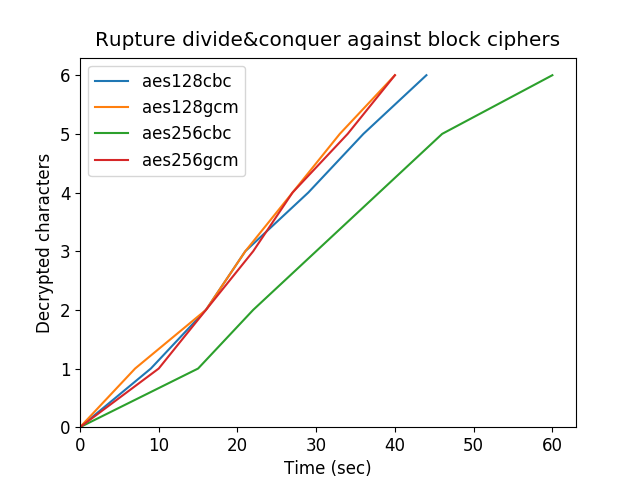
\includegraphics[width=0.48\textwidth]{experiments/rupture_performance/rupture_div_conq_performance.png}
       \caption{Rupture divide and conquer performance}
      \label{fig:rupture_performance_div_conq}
   \end{figure}

As can be seen, we were able to decrypt all 6 unknown characters of the word in
all cases. The total time for decrypting the characters ranged from 40 seconds,
in the case of GCM mode, to 60 seconds, in the case of CBC mode with 256-bit
block size. Therefore the average time for decrypting a single character using
the divide and conquer method was 6-10 seconds.

In our second experiment we tested the consistency of Rupture by targeting a
longer secret. This time the secret was 25 characters and we used the
serial method for computing the reflections. The rest of the experiment
parameters were the same as before. The results of this experiments are shown in
Figure \ref{fig:rupture_performance_serial}.

   \begin{figure}[thpb]
      \centering
          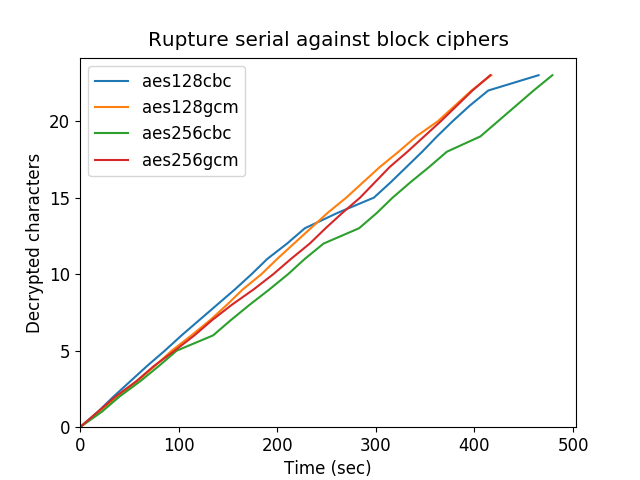
\includegraphics[width=0.48\textwidth]{experiments/rupture_performance/rupture_serial_performance.png}
      \caption{Rupture serial performance}
      \label{fig:rupture_performance_serial}
   \end{figure}

We were again able to decrypt all unknown characters in all AES modes and block
sizes. This time the total time ranged from 416 (GCM-256) to 479 (CBC-256)
seconds. Therefore the average time for decrypting a single character using the
serial method was 18-21 seconds.

We also notice that Rupture performs slightly worse against AES CBC compared to
AES GCM regardless of the block size. Further investigation on how different
modes affect the attack's performance should be conducted in future work.
